\tocsection{\textbf{9/10/26 Lecture 5:} More on Sufficiency}

Recall that if $X_1, X_2 \overset{\tt{iid}}{\sim} \tt{Binom}(n, \theta)$, then $X_1 + X_2$ is a sufficient statistics. However, if $X_1, X_2 \iidsim e^{-\abs{x - n\theta}}$, then it turns out $X_1 + X_2$ aren't sufficient statistics.\\

However, in the above two cases, both $(X_{(1)}, X_{(2)})$ are sufficient. Notice that this is due to the fact they are independent and identically distributed, so that are exchangeable (just rename one to the other). Thus, we can conclude that if $X_1, X_2$ are $\iidsim$, then $(X_{(1)}, X_{(2)})$ is sufficient! Consider the following diagram for a sufficient statistic $T$. 

\begin{center}
    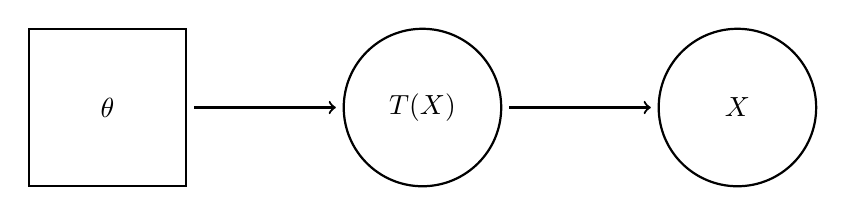
\begin{tikzpicture}

        \draw[thick, black] (-5, -1) -- (-5, 1) -- (-3, 1) -- (-3, -1) -- cycle;
        \node at (-4, 0) {$\theta$};

        \draw[thick, black] (0, 0) circle (1);
        \node at (0, 0) {$T(X)$};

        
        \draw[thick, black] (4, 0) circle (1);
        \node at (4, 0) {$X$};

        \draw[thick, ->] (-2.9, 0) -- (-1.1, 0);
        \draw[thick, ->] (1.1, 0) -- (2.9, 0);

    \end{tikzpicture}
\end{center}
That is, knowing $\theta$ tells you the distribution of $T(X)$, and knowing $T(X)$ tells you the distribution of $X$. Thus, in a sense, knowing all of $X$ is pointless, we just need to know $T(X)$.\\

A funny but effective way of remembering this is that, if a group of scientists give you the data $X$, and you compute $T(X)$ and accidentally throw out $X$, then if the scientists ask you for the data you can generate your own sample $\tilde{X}$ with $T(X)$ and no one would ever be able to tell you lost your data.\\

What this also means is that if we have a sufficient statistics $T$, then we should have our estimators be functions of $T$ as using $X$ just introduces unnecessary randomness from the conditional distribution of $X$ given $T$ (which we would know). This is what is called a \emph{sufficiency reduction}: just using $T(X)$ instead of $X$. 

\subsection*{Order Statistics}
\sectionspace

\begin{definition}[\textbf{Definition 5.1}: Order Statistics]
    For $X = (X_1, X_2, \ldots, X_n) \in \R^n$, define the \emph{order statistics} of $X$ to be
    \[ \min_{i} X_i = X_{(1)} \leq X_{(2)} \leq \cdots \leq X_{(n)} = \max_{i} X_i \]
    where $\{X_{(1)}, \ldots, X_{(n)}\} = \{x_1, \ldots, x_n\}$. 
\end{definition}

Now, if $X_1, \ldots, X_n \iidsim P_{\theta}$, and $\cal{P} = \{P_{\theta}^{n} \col \theta \in \Theta\}$ is any model, then due to the invariance of $X_1, \ldots, X_n$ under permutations, this immediately implies the statistics $(X_{(i)})_{i = 1}^{n} = (X_{(1)}, \ldots, X_{(n)})$ is sufficient. Thus, there is a correspondence
\[ (X_{(i)}) \text{ is sufficient} \iff \tt{ model is symmetric} \]

\subsection*{Empirical Distribution}
\sectionspace

\begin{definition}[\textbf{Definition 5.2:} The Dirac Measure]
    Define the \emph{Dirac measure} to be $\delta_{x}(A) = 1\{x \in A\}$ for some $x \in A$. The \emph{empirical distribution} is, given random variables, $X_1, \ldots, X_n$
    \[ \hat{P}_{n}(\cdot) = \frac{1}{n}\sum_{i = 1}^{n} \delta_{X_{i}}(\cdot) \]
    so $\hat{P}_{n}(A) = \#\{i : X_{i} \in A\}/n$. Notice that $\hat{P}_{n}(\cdot)$ is a random measure, depending on the $X_1, \ldots, X_n$. 
\end{definition}
Given iid $X_1, \ldots, X_n$, since the multiset $\{X_1, \ldots, X_n\}$ is sufficient, we see that $\hat{P}_{n}$, which tells you the multiset, is also sufficient.\\

Now, lets move on to minimal sufficiency. Notice that if $X_1, X_2 \iidsim \Binom(n, \theta)$, then $X = (X_1, X_2)$ is sufficient, $(X_{(1)}, X_{(2)})$ is sufficient, and so is $X_1 + X_2$.\\

However, notice that given $(X_1, X_2)$, we can generate $S(X) = (X_{(1)}, X_{(2)})$, and given $(X_{(1)}, X_{(2)})$, we can generate $T(X) = X_1 + X_2$. Thus, this gives us a diagram

\begin{center}
    \begin{tikzcd}
        & X \arrow[d] \arrow[ldd, out = 200, in = 80] \arrow[rdd, out = -20, in = 100] & \\
        & S(X) \arrow[dr] \arrow[dl] & \\ 
        T(X) \arrow[rr, leftrightarrow] & & \overline{X}
    \end{tikzcd}
\end{center}
where $\overline{X} = \frac{X_1 + X_2}{2}$. The arrows that connect two sufficient statistics tells us that we can compute one statistic from the other. That is, $A \rightarrow B$ implies $B = f(A)$. Thus, this allows us to define what a minimally sufficient statistic is. First, a quick proposition:

\begin{lemma}[\textbf{Proposition 5.3}]
    If $T(X)$ is sufficient and $T(X) = f(S(X))$, then $S(X)$ is sufficient.
\end{lemma}
\begin{proof}{Proof:}
    We use the factorization theorem, noting 
    \[ p_{\theta}(x) = g_{\theta}(T(x))h(x) = (g_{\theta} \circ f)(S(x))h(x) \]
    which tells us that $S(X)$ is sufficient. 

    $\qed$
\end{proof}

\begin{definition}[\textbf{Definition 5.4:} Minimal Sufficient Statistic]
    A sufficient statistic $T(X)$ is \emph{minimal sufficient} if
    \begin{enumerate}
        \item $T(X)$ is sufficient.
        \item If $S(X)$ is sufficient, then $T(X) = f(S(X))$ for some $f$. 
    \end{enumerate}
\end{definition}

\subsection*{Bayesian Interpretation of Sufficiency}
\sectionspace

Consider a model $\cal{P} = \{p_{\theta} : \theta \in \Theta\}$, a prior $\theta \sim \pi$, and data $x \given \theta \sim p_{\theta}$. Then, we see that
\[ \pi(\theta \given x) = \frac{\pi(\theta)p_{\theta}(x)}{\int \pi(\gamma)p_{\gamma}(x)d\gamma} \]
then, if $T$ is sufficient, we see that
\begin{align*}
    \frac{\pi(\theta)p_{\theta}(x)}{\int \pi(\gamma)p_{\gamma}(x)d\gamma} &= \frac{\pi(\theta)g_{\theta}(T(x))h(x)}{\int_{\gamma}\pi(\gamma)g_{\gamma}(T(x))h(x)d\gamma}\\
    &= \frac{\pi(\theta)g_{\theta}(T(x))}{\int \pi(\gamma)g_{\gamma}(T(x))d\gamma}
\end{align*}
Thus, we see that the value of $T(x)$ determines our posteriors $\pi(\theta \given x)$. Thus, what sufficiency does in this case is collapsing what are ``equivalent'' (give the same posterior) data sets.\\

Now, we know that $\pi(\theta \given x) \propto_{\theta} \pi(\theta)p_{\theta}(x)$, which implies that $\pi(\theta \given x) = \pi(\theta \given y)$ if, and only if, $\frac{p_{\theta}(x)}{p_{\theta}(y)}$ is constant in $\theta$. Thus, changing $\theta$ does not change this likelihood ratio, which means that if $x$ and $y$ have the same sufficient statistic, this ratio is constant over $\theta$.\\

Now, heuristically, we see that a typical sufficient statistic collapses data, but it doesn't maximally collapse data, which is what a maximal sufficient statistic would do. This, along with the above insight can tell us a necessary and sufficient condition for minimally sufficient statistics.\\

First, assuming that $\cal{P}$ has densities $p_{\theta}$ on a sample space $X$, we can define an equivalence relation
\[ x \equiv_{p} y \text{ iff } \frac{p_{\theta}(x)}{p_{\theta}(y)} \text{ does not depend on } \theta \]
First, notice that if $T(x) = T(y)$, then $x \equiv_{p} y$ from above. Now, consider the map $C$ that sends $x$ to it's equivalence class under $\equiv_{p}$. Under some mild conditions, we can show that this is a sufficient statistics. Also, as $T(x) = T(y) \implies x \sim_{p} y \implies C(x) = C(y)$, we see that we can write $C(x) = f(T(x))$. As this holds for all sufficient statistics, this implies that $C$ is minimal!

\begin{theorem}[\textbf{Theorem 5.5 (Bahader)}]
    $T(X)$ is minimal sufficient if $x \equiv_{p} y \iff T(x) = T(y)$. That is, the equivalence relation induced by $T$ is $\equiv_{p}$. 
\end{theorem}

Now, lets see how we can find these minimal sufficient statistics.

\begin{definition}[\textbf{Definition 5.6:} Likelihood Functions]
    Assume $\cal{P} = \{P_\theta : \theta \in \Theta\}$ has densities $p_{\theta}$. The \emph{likelihood function} is $\tt{Lik}(\theta; X) = p_{\theta}(X)$, which is a random function of $\theta$. The \emph{log-likelihood function} is $\ell(\theta; X) = \log p_{\theta}(X)$. 
\end{definition}

Now, notice that as
\[ x \equiv_{\theta} y \iff \ell(\theta; x) - \ell(\theta; y) \text{ is constant in } \theta \]
Thus, we see that the equivalence classes of $\ell(\theta; X)$ up to scaling are minimal sufficient by Theorem 5.5! What this also means is that $T(X)$ is minimal sufficient if $\ell(\theta;x) - \ell(\theta;y)$ is constant in $\theta$ if, and only if, $T(x) = T(y)$.
